% !TEX root = ../thesis.tex


\chapter{Appendix}
\section{DMD}
\subsection{Theory -- Floyd-Steinberg Dithering}
\vfill
\begin{algorithm}
    \caption{The Floyd-Steinberg Dithering Algorithm}
    \label{alg:floyd_steinberg}
    %
    \begin{algorithmic}[1]
        \Require A greyscale (0 to 1) image with dimensions $X \times Y$
        \Ensure A binary (black and white) image with the same dimensions
        \Procedure{FloydSteinberg}{Image}
        \ForAll {$0 \leq j < Y$}
        \ForAll {$0 \leq i < X$}
        \State Old $\gets$ Image[$i$, $j$]
        \State New $\gets$ \Call{Round}{Old}
        \State Error $\gets$ Old $-$ New
        \State Image[$i + 1$, $j\negphantom{j}\phantom{j + 1}$] $\gets$ Image[$i + 1$, $j\negphantom{j}\phantom{j + 1}$] $+\ \text{Err}\times 7/16$
        \State Image[$i - 1\negphantom{i-1}\phantom{i+1}$, $j + 1$] $\gets$ Image[$i - 1\negphantom{i-1}\phantom{i+1}$, $j + 1$] $+\ \text{Err}\times 3/16$
        \State Image[$i\negphantom{i}\phantom{i+1}$, $j + 1$] $\gets$ Image[$i\negphantom{i}\phantom{i+1}$, $j + 1$] $+\ \text{Err}\times 5/16$
        \State Image[$i + 1$, $j + 1$] $\gets$ Image[$i + 1$, $j + 1$] $+\ \text{Err}\times 1/16$
        \EndFor
        \EndFor
        \EndProcedure
    \end{algorithmic}
\end{algorithm}
\vfill

\pagebreak
\subsection{Results -- Sinusoidal Fringes as Artificial Deviation}
\vfill
\begin{minipage}{\linewidth}
    \centering
    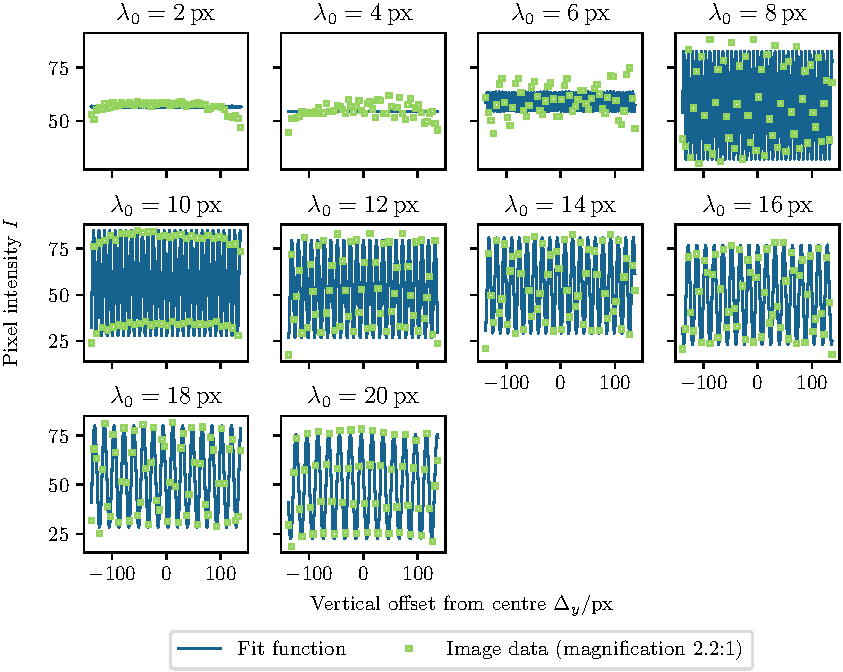
\includegraphics[]{DMD/Results/LengthScaleOld}
    \captionof{figure}[Sinusoidal modulation pattern images with fits]{From the image data, only every fifth value is plotted for better visibility. $\lambda_0$ is the period of the sinusoidal pattern that has been added as a deviation. The offset in intensity is a result of a wrong setting for the edge detection range, which had been set to only $r=\SI{7}{px}$.}
    \label{fig:dmd_results_resolution_cuts_old}
\end{minipage}
\vfill
\pagebreak

\noindent\begin{minipage}[c][\textheight][c]{\linewidth}
    \centering
    \includegraphics[]{DMD/Results/LengthScale}
    \captionof{figure}[Sinusoidal modulation pattern images with fits]{From the image data, only every fifth value is plotted for better visibility. $\lambda_0$ is the period of the sinusoidal pattern that has been added as a deviation. The offset in intensity is a result of a wrong setting for the edge detection range, which had been set to only $r=\SI{7}{px}$.}
    \label{fig:dmd_results_resolution_cuts}
\end{minipage}
% \pagebreak



\section{Evaporation}
\subsection{Theory -- Derivation of the Density of States}
\label{sec:appendix_dos}
We consider the power-law potential
\[
    U(\vec{r}) = U_x \left| \frac{x}{x_0} \right|^{\alpha_x} + U_y \left| \frac{y}{y_0} \right|^{\alpha_y} + U_z \left| \frac{z}{z_0} \right|^{\alpha_z}.
\]
The general density of states is \cite{PhysRevA.35.4354}
\begin{equation*}
    D(E) = \frac{2\pi(2m)^\frac{3}{2}}{(2\pi\hbar)^3} \underbrace{\int_{V^*(E)} \sqrt{E - U(\vec{r})}\multidiff{3}{r}}_{\equiv I(E)}
\end{equation*}
where $V^*(E)$ is the volume where $U(\vec{r}) < E$. Because the potential is symmetric along all axes, we can simplify the integration over one octant:
\begin{equation*}
    I(E) = 8\int_0^{\tilde{x}} \int_0^{\tilde{y}} \int_0^{\tilde{z}} \diff{z} \diff{y} \diff{x} \sqrt{E - U_x \left(\frac{x}{x_0}\right)^{\alpha_x} - U_y \left(\frac{y}{y_0}\right)^{\alpha_y} - U_z \left(\frac{z}{z_0}\right)^{\alpha_z}}
\end{equation*}
with
% \begin{align*}
%     \tilde{x} &= x_0 \left(\frac{E}{U_x}\right)^{\frac{1}{\alpha_x}}, \\ 
%     \tilde{y} &= y_0 \left(\frac{E - U_x\left(\frac{x}{x_0}\right)^{\alpha_x}}{U_y}\right)^{\frac{1}{\alpha_y}}, \\ 
%     \tilde{z} &= z_0 \left(\frac{E - U_x\left(\frac{x}{x_0}\right)^{\alpha_x} - U_y\left(\frac{y}{y_0}\right)^{\alpha_y} }{U_z}\right)^{\frac{1}{\alpha_z}}. 
% \end{align*}
\begin{equation*}
    \tilde{x} = x_0 \left(\frac{E}{U_x}\right)^{\frac{1}{\alpha_x}},
    \,\, 
    \tilde{y} = y_0 \left(\frac{E - U_x\left(\frac{x}{x_0}\right)^{\alpha_x}}{U_y}\right)^{\frac{1}{\alpha_y}},
    \,\,
    \tilde{z} = z_0 \left(\frac{E - U_x\left(\frac{x}{x_0}\right)^{\alpha_x} - U_y\left(\frac{y}{y_0}\right)^{\alpha_y} }{U_z}\right)^{\frac{1}{\alpha_z}}. 
\end{equation*}
We will substitute variables twice, in order not to skip too many substeps. First we substitute
\begin{equation*}
    \zeta^{\alpha_x} = U_z \left(\frac{z}{z_0}\right)^{\alpha_z}, \quad \xi^{\alpha_y} = U_y \left(\frac{y}{y_0}\right)^{\alpha_y}, \quad
    \chi^{\alpha_x} = U_x \left(\frac{x}{x_0}\right)^{\alpha_x}
\end{equation*}
to get
\begin{equation*}
    I(E) = \frac{8 x_0 y_0 z_0}{U_x^{1/\alpha_x} U_y^{1/\alpha_y} U_z^{1/\alpha_z}} \int_0^{\tilde{\chi}} \int_0^{\tilde{\xi}} \int_0^{\tilde{\zeta}} \diff{\zeta} \diff{\xi} \diff{\chi} \sqrt{E - \chi^{\alpha_x} - \xi^{\alpha_y} - \zeta^{\alpha_z}}
\end{equation*}
where we have introduced the new quantities
\begin{equation*}
    \tilde{\chi} = E^{1/\alpha_x}, \quad \tilde{\xi} = \left(E - \chi^{\alpha_x}\right)^{1/\alpha_y}, \quad \tilde{\zeta} = \left(E - \chi^{\alpha_x} - \xi^{\alpha_y}\right)^{1/\alpha_z}.
\end{equation*}
Now we substitute
\begin{equation*}
    u = \frac{\chi}{E^{1/\alpha_x}}, \quad v = \frac{\xi}{\left(E - \chi^{\alpha_x}\right)^{1/\alpha_y}}, \quad w = \frac{\zeta}{\left(E - \chi^{\alpha_x} - \xi^{\alpha_y}\right)^{1/\alpha_z}}
\end{equation*}
and we arrive at
\begin{align*}
    I(E) &= \frac{8 x_0 y_0 z_0}{U_x^{1/\alpha_x} U_y^{1/\alpha_y} U_z^{1/\alpha_z}} E^{\frac{1}{2} + \frac{1}{\alpha_x} + \frac{1}{\alpha_y} + \frac{1}{\alpha_z}} \\
    &\phantom{=} \times \underbrace{\int_0^1 \diff{u} \left(1 - u^{\alpha_x}\right)^{\frac{1}{2} + \frac{1}{\alpha_y} + \frac{1}{\alpha_z}} \int_0^1 \diff{v} \left(1 - v^{\alpha_y}\right)^{\frac{1}{2} + \frac{1}{\alpha_z}} \int_0^1 \left(1 - w^{\alpha_z}\right)^\frac{1}{2}}_{\equiv X(\alpha_x,\alpha_y,\alpha_z)}.
\end{align*}
The integral
\[
    \int_0^1 \diff{\tau} \left(1 - \tau^a\right)^b 
\]
can be related to the beta function $\text{B}(x,y)$ \cite[Eq.~5.12.1]{NIST:DLMF} by substituting $t = \tau^a$
\begin{equation*}
    \int_0^1 \diff{\tau} \left(1 - \tau^a\right)^b = \frac{1}{a} \int_0^1 \diff{t}\, t^{\frac{1}{a} - 1} \left(1 - t\right)^{(b + 1) - 1} =\frac{1}{a} \text{B}\!\left(\frac{1}{a}, b + 1\right).
\end{equation*}
Using this simplifies $X(\alpha_x,\alpha_y,\alpha_z)$ to 
\begin{equation*}
    X(\alpha_x,\alpha_y,\alpha_z) = \frac{1}{\alpha_x \alpha_y \alpha_z} \text{B}\!\left(\frac{1}{\alpha_x}, \frac{3}{2} + \frac{1}{\alpha_y} + \frac{1}{\alpha_z} \right) \cdot \text{B}\!\left(\frac{1}{\alpha_y}, \frac{3}{2} + \frac{1}{\alpha_z} \right) \cdot \text{B}\!\left(\frac{1}{\alpha_z}, \frac{3}{2}\right).
\end{equation*}
We can simplify this even further by using the relation of the Beta function to the Gamma function:
\begin{equation*}
    \text{B}(x,y) = \frac{\Gamma(x)\Gamma(y)}{\Gamma(x + y)}
\end{equation*}
\begin{align*}
    \Rightarrow \quad X(\alpha_x,\alpha_y,\alpha_z) &= \frac{1}{\alpha_x \alpha_y \alpha_z} \frac{\Gamma\!\left(\frac{1}{\alpha_x}\right) \Gamma\!\left(\frac{3}{2} + \frac{1}{\alpha_y} + \frac{1}{\alpha_z}\right)}{\Gamma\!\left(\frac{3}{2} + \frac{1}{\alpha_x} + \frac{1}{\alpha_y} + \frac{1}{\alpha_z}\right)} \frac{\Gamma\!\left(\frac{1}{\alpha_y}\right) \Gamma\!\left(\frac{3}{2} + \frac{1}{\alpha_z}\right)}{\Gamma\!\left(\frac{3}{2} + \frac{1}{\alpha_y} + \frac{1}{\alpha_z}\right)} \frac{\Gamma\!\left(\frac{1}{\alpha_z}\right) \Gamma\!\left(\frac{3}{2}\right)}{\Gamma\!\left(\frac{3}{2} + \frac{1}{\alpha_z}\right)} \\
    &= \frac{1}{\alpha_x \alpha_y \alpha_z} \frac{\Gamma\!\left(\frac{1}{\alpha_x}\right) \Gamma\!\left(\frac{1}{\alpha_y}\right) \Gamma\!\left(\frac{1}{\alpha_z}\right) \Gamma\!\left(\frac{3}{2}\right)}{\Gamma\!\left(\frac{3}{2} + \frac{1}{\alpha_x} + \frac{1}{\alpha_y} + \frac{1}{\alpha_z}\right)} \qquad \Big| \, x\Gamma(x) = \Gamma(x + 1) \\
    &= \frac{\sqrt{\pi}}{2}\cdot\frac{\Gamma\!\left(1 + \frac{1}{\alpha_x}\right) \Gamma\!\left(1 + \frac{1}{\alpha_y}\right) \Gamma\!\left(1 + \frac{1}{\alpha_z}\right)}{\Gamma\!\left(\frac{3}{2} + \frac{1}{\alpha_x} + \frac{1}{\alpha_y} + \frac{1}{\alpha_z}\right)} \\
    &\equiv \frac{\sqrt{\pi}}{2} \times \frac{F(\alpha_x,\alpha_y,\alpha_z)}{\Gamma(\xi)}
\end{align*}
where
\begin{equation*}
    F(\alpha_x,\alpha_y,\alpha_z) = \Gamma\!\left(1 + \frac{1}{\alpha_x}\right) \Gamma\!\left(1 + \frac{1}{\alpha_y}\right) \Gamma\!\left(1 + \frac{1}{\alpha_z}\right),
    \quad
    \xi = \frac{3}{2} + \frac{1}{\alpha_x} + \frac{1}{\alpha_y} + \frac{1}{\alpha_z}.
\end{equation*}
So finally, the complete density of states is given by
\begin{equation*}
    D(E) = \left(\frac{2m}{\pi\hbar^2}\right)^\frac{3}{2} \frac{x_0 y_0 z_0}{U_x^{1/\alpha_x} U_y^{1/\alpha_y} U_z^{1/\alpha_z}} \frac{F(\alpha_x,\alpha_y,\alpha_z)}{\Gamma(\xi)} \times E^{\xi - 1}.
\end{equation*}

\vfill
\subsection{Implementation -- Custom Adaptive Runge-Kutta}
\begin{algorithm}
    \caption{Particle Movement Procedure with Adaptive Runge-Kutta Method}
    \label{alg:dsmc_movement_impl}
    %
    \begin{algorithmic}[1]
    \Require \Dt, the timestep to propagate each particle forward by
    \Procedure {MoveStep}{\Dt}
    \newcommand*{\TOL}{\ensuremath{\Delta_\text{tolerance}}\xspace}
    \State $\TOL = \num{e-7}$ \Comment{tolerance parameter}
    \ForAll {particles $i \in$ cloud}
    \State $t \gets 0$ \Comment{time passed}
    \State $\Dt_\text{local} \gets \min (\classprop{i}{\delta t}, \Dt)$ \Comment{local timestep}
    \While {$t < \Dt$}
    \State $\{K[0], L[0]\} \gets \Dt_\text{local}\cdot \{ \Call{Force}{\classprop{i}{\vec{r}}}/m , \classprop{i}{\vec{v}}  \}$
    \State $\{K[1], L[1]\} \gets \Dt_\text{local}\cdot \{ \Call{Force}{\classprop{i}{\vec{r}} + 0.5\cdot L[0]}/m , \classprop{i}{\vec{v}} + 0.5\cdot K[0]  \}$
    \State $\{K[2], L[2]\} \gets \Dt_\text{local}\cdot \{ \Call{Force}{\classprop{i}{\vec{r}} + 0.5\cdot L[1]}/m , \classprop{i}{\vec{v}} + 0.5\cdot K[1]  \}$
    \State $\{K[3], L[3]\} \gets \Dt_\text{local}\cdot \{ \Call{Force}{\classprop{i}{\vec{r}} + L[2]}/m , \classprop{i}{\vec{v}} + K[2] \}$
    \Statex
    \State $\vec{r}' \gets \classprop{i}{\vec{r}} + 1/6\cdot(L[0] + 2\cdot L[1] + 2\cdot L[2] + L[3])$
    \State $\vec{v}' \gets \classprop{i}{\vec{v}} + 1/6\cdot(K[0] + 2\cdot K[1] + 2\cdot K[2] + K[3])$
    \Statex
    \State $E_0 \gets m/2 \cdot (\classprop{i}{\vec{v}})^2 + \Call{Potential}{\classprop{i}{\vec{r}}}$ \Comment{total energy before}
    \State $E \gets m/2 \cdot (\vec{v}')^2 + \Call{Potential}{\classprop{i}{\vec{r}'}}$ \Comment{total energy after}
    \State $\Delta E \gets$ \Ternary{$E_0 \neq 0$}{$|E-E_0|/E_0$}{$\num{0.999}\cdot \TOL$}
    \Statex
    \If {$\Delta E < \TOL$}
    \State $t \gets t + \Dt_\text{local}$ \Comment{advance the time tracker}
    \State $\{\classprop{i}{\vec{r}}, \classprop{i}{\vec{v}}\} \gets \{\vec{r}', \vec{v}'\}$ \Comment{apply the changes in position and velocity}
    \EndIf
    \Statex
    \State $\Dt_\text{local} \gets \Dt_\text{local}\cdot$ \Ternary{$\Delta E \neq 0$}{$0.9 \cdot (\TOL / \Delta E)^{\num{0.25}}$}{$10$}
    \Statex
    \If {$t + \Dt_\text{local} > \Dt$}
    \State $\classprop{i}{\delta t} \gets \Dt_\text{local}$ \Comment{update local timestep of this particle}
    \State $\Dt_\text{local} \gets \Dt - t$ \Comment{do not go beyond \Dt}
    \EndIf
    \EndWhile
    \EndFor
    \EndProcedure
    \end{algorithmic}
\end{algorithm}
\vfill

\pagebreak
\subsection{Tests and Results -- Derivation of the Mean Scattering Rate}
\label{sec:appendix_average}
The mean scattering rate in a gas is given by
\begin{equation*}
    \langle \Gamma \rangle = \langle n \sigma \crel \rangle = \langle n \rangle \cdot \meanProb.
\end{equation*}
To find the value of \meanProb{}, we need to average over the Maxwell-Boltzmann distributions for both collision partners.
\begin{align*}
    \meanProb &= \iint \multidiff{3}{c_1} \multidiff{3}{c_2}\; \frac{8\pi a^2\crel}{1 + a^2 k^2} \times n(\vec{c}_1) n(\vec{c}_2) \\
    &= \frac{8\pi a^2}{(2\pi m \kB T)^3}\iint \multidiff{3}{c_1} \multidiff{3}{c_2}\; \frac{\crel}{1 + a^2 k^2} \exp\!\left(-\frac{m(\vec{c}_1^2 + \vec{c}_2^2)}{2\kB T}\right) 
    \intertext{We can now change variables to centre-of-mass and relative coordinates and integrate out the angular part}
    &= (4\pi)^2 \frac{8\pi a^2}{(2\pi m \kB T)^3}\int_0^\infty \diff{\crel}\; \crel^2 \frac{\crel}{1 + a^2 k^2} \exp\!\left(-\frac{m\crel^2}{4\kB T}\right) \nonumber \\
    &\phantom{=} \quad \times \int_0^\infty \diff{c_\text{COM}}\; c_\text{COM}^2 \exp\!\left(-\frac{mc_\text{COM}^2}{\kB T}\right) \\
    &= 4\sqrt{\pi} a^2 \left(\frac{m}{\kB T}\right)^\frac{3}{2} \int_0^\infty \diff{\crel} \frac{\crel^2}{1 + a^2 \frac{m^2 \crel^2}{4\hbar^2}} \exp\!\left(-\frac{m\crel^2}{4\kB T}\right)
    \intertext{where we have performed the integration over $c_\text{COM}$ and used the relation $k = \frac{m\crel}{2\hbar}$. Making the integral dimensionless and introducing the (also dimensionless) parameter $\chi = \sqrt{\frac{\hbar^2}{a^2 m \kB T}}$ we find}
    &= 64\sqrt{\pi} \cdot \frac{a\hbar}{m} \cdot \chi \int_0^\infty \diff{u}\; \frac{u^3}{\chi^2 + u^2} \exp(-u^2) \\
    &= 32\sqrt{\pi} \cdot \frac{a\hbar}{m} \cdot \chi \left(1 + \chi^2\exp(\chi^2)\text{Ei}(-\chi^2)\right)
    \intertext{where Ei is the exponential integral \cite[Eq.~6.2.5]{NIST:DLMF}. Because $\chi^2$ can be much larger than 1, for calculation on a computer it is better to express this using the confluent hypergeometric function $U$ \cite[Eq.~13.2.6]{NIST:DLMF}:}
    \meanProb &= 32\sqrt{\pi} \cdot \frac{a\hbar}{m} \cdot \chi \left(1 + \chi^2U(1,1,\chi^2)\right).
\end{align*}

\pagebreak
\subsection{Tests and Results -- Evaporation Trajectories, Cases 1--4}
\vfill
\noindent\begin{minipage}[c]{\linewidth}
    \centering
    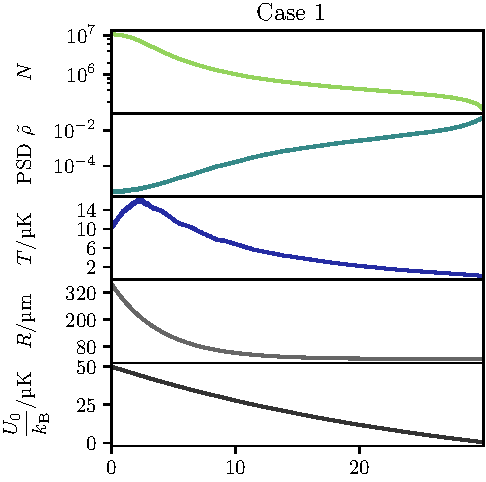
\includegraphics[]{Evap/Trajectory-Results-1}\hfill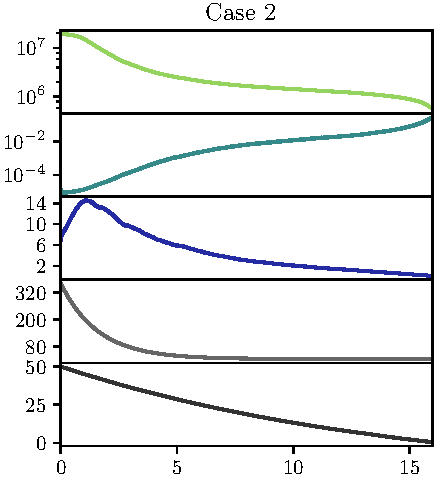
\includegraphics[]{Evap/Trajectory-Results-2.pdf} \\[\baselineskip]
    \noindent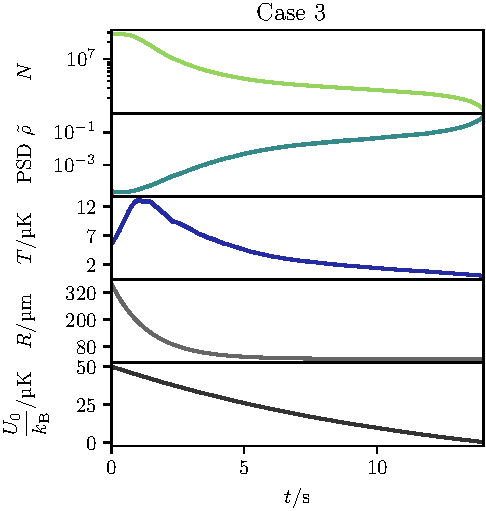
\includegraphics[]{Evap/Trajectory-Results-3}\hfill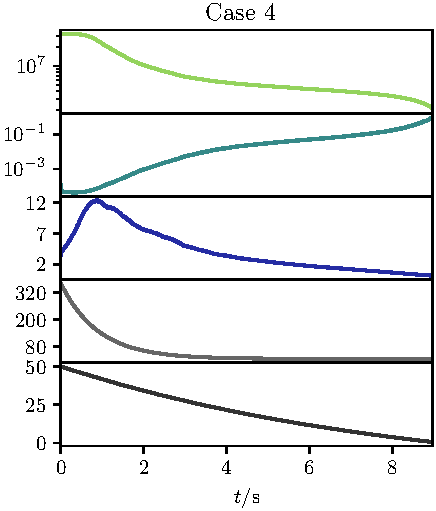
\includegraphics[]{Evap/Trajectory-Results-4.pdf}
    \captionof{figure}[Evaporation trajectories for the cases 1--4 defined in \cref{sec:eva_test}]{The initial and final values for the parameters shown here are listed in \cref{tab:evap_results}. The atom number and phase space density axes are logarithmic, the others linear.}
    \label{fig:eva_cases14}
\end{minipage}
\vfill